
\begin{multicols*}{2}

\section{Arcanist}

\lettrine[lines=3, lhang=0.15, loversize=0.25, findent=.5em]{A}{rcanists} are cloistered scholars that have spent years studying ley lines and the patterns of magic. They have learned to weave these lines ans shape reality according to their will. 

\subsection*{Spell Shield}

When you are hit by an attack or targeted by the magic missile spell, you can spend your reaction to create an invisible barrier of magical force to appear and protect you. Spend a mana die, until the start of your next turn, you have a +5 bonus to AC, including against the triggering attack, and you take no damage from magic missile.


\subsection*{Metamagic}

At 3rd level, you gain the ability to twist your spells to suit your needs. Refer to the arcanists's metamagic table for details.

The more powerful the metamagic, the more instability there is in successfully applying it to a spell. For example, there is always a risk that you won't sculpt a spell to protect all your allies.

You can use only one Metamagic option on a spell when you cast it, unless otherwise noted.



\subsection*{High-Weaver}

At 7th level, you have achieved such mastery over certain spells that you can cast them at will. Choose two 1st-level arcanist spels. You can cast those spells at their lowest level without expending a spell slot. If you want to cast either spell at a higher level, you must expend a spell slot as normal.

Additionally, apply one of the effect of the high-weave table to your high weave spells.


\textbf{Named Spell:} Add your name as a suffix or prefix to your high weave spells. For example, if Maya has choose 
magic missle as her high weave, people around the world might start to recognize it as Maya's magic missile. 


\textbf{Cosmetic Changes:} Discuss with your DM any cosmetic changes that distinguish your high weave spells from mudane ones, e.g., Maya's magic missiles are three green darts always floating around her head like a corona. At her command, the darts fly towards a target and a few seconds after, new darts appear.



\subsection*{Syphon-Weave}

The weave is nothing more than a source of magical restoration for you. You can disrupt it an recover energy. Lore tells that areas of dead magic are the result of power-hungry syphon-weavers.

At 9th level, you can use your bonus action to regain all your mana points. 

Once you use this feature, you can’t use it again until you finish a long rest.




\begin{Figure}
\centering
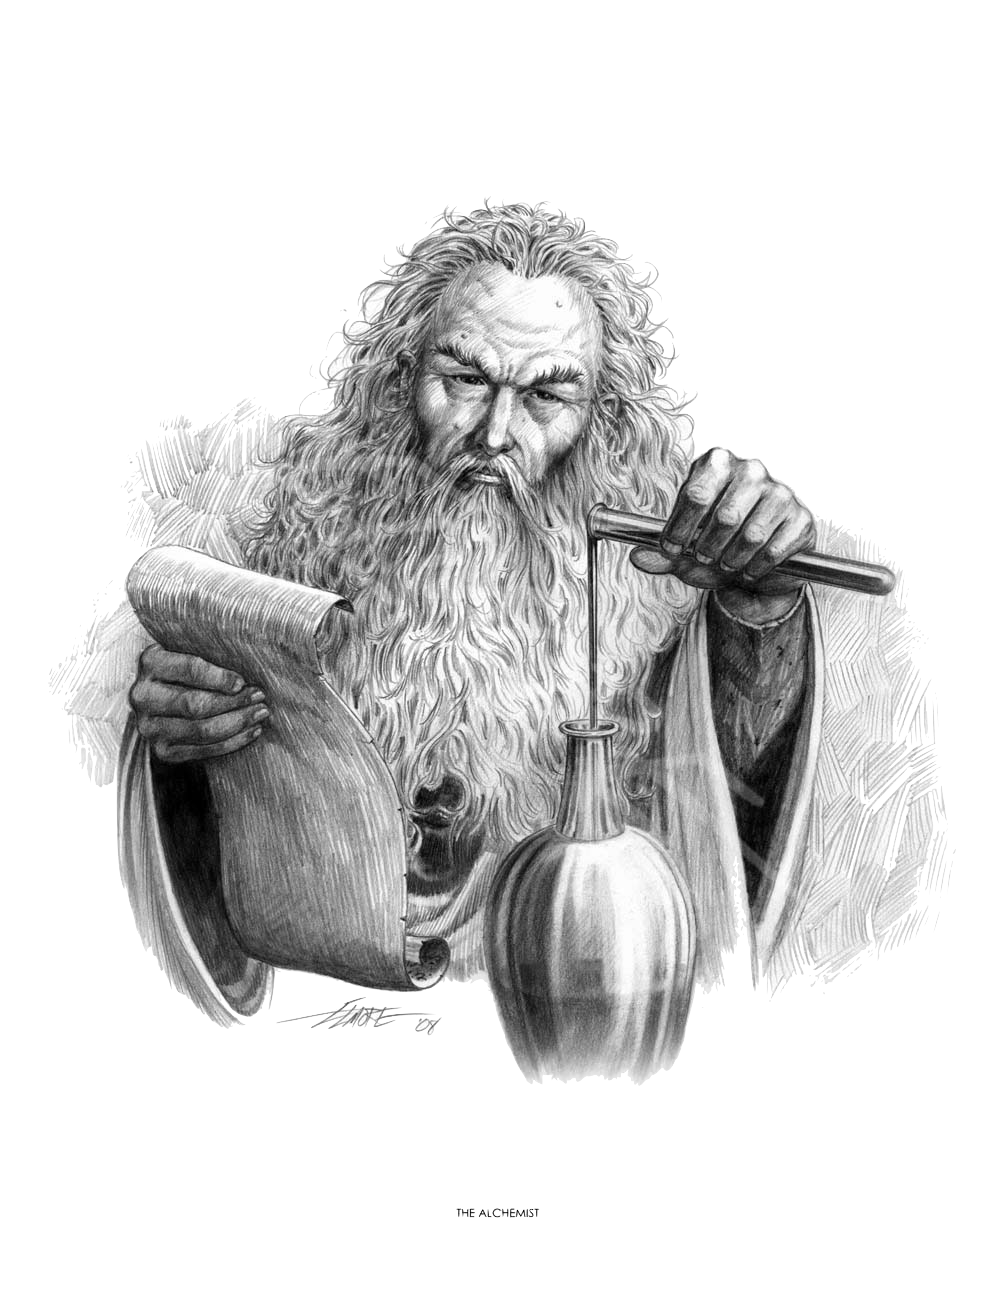
\includegraphics[width=\textwidth]{img/wizard.png}
{\scriptsize Art by Larry Elmore}
\end{Figure}



\header{High Weave Effects}
\begin{rpg-table}
	Deadly & Add your mana die as extra damage to one creature hit by the spell.
	\\
	Warding & A spell that requires concentration or that has a fixed duration (e.g., Mage Armor) and that targets you or an ally grants temporary hit points equal to your mana die + your spellcasting ability modifier
	\\
	Execrate & The first time a creature succeeds on a save against your spell, roll your mana die. On a 1 or 2, the creature fails. This effect applies only once per spell. \\
\end{rpg-table}	
    
\end{multicols*}


\clearpage

\begin{table}[ht!]
\begin{small}
\rowcolors{2}{}{commentgreen}
\begin{center}
\begin{tabular}{ll}
\multicolumn{2}{l}{\parbox[l][0.6cm][c]{15cm}{\textbf{Arcanist Metamagic}}} 
\\
\hline 
\textbf{Name} & \parbox[l][0.6cm][c]{15cm}{\textbf{Description}}
\\ 
Sculpt Spells & \parbox[l][2.8cm][c]{15cm}{
When you cast a spell that forces other creatures to make a saving throw, you can protect some of those creatures from the spell’s full force. To do so, you spend 1 mana point and choose a number of those creatures up to your mana die (minimum of one creature). The chosen creatures automatically succeed on their saving throws against the spell, and they take no damage if they would normally take half damage on a successful save.
}
\\ 
Distant Spell & \parbox[l][2.2cm][c]{15cm}{
When you cast a spell that has a range of 5 feet or greater, you can spend 1 mana point to increase the range of the spell by 10 feet times your rolled mana die.
\\
When you cast a spell that has a range of touch, you can spend 1 mana point to make the range of 10 feet times your rolled mana die.
}
\\ 
Empowered Spell & \parbox[l][2.8cm][c]{15cm}{
When you roll damage for a spell, you can spend 1 mana point to reroll a number of the damage dice equal to your rolled mana die. You must use the new rolls. Additionally, you add one mana die to the damage of the spell.
\\
You can use Empowered Spell even if you have already used a different Metamagic option during the casting of the spell.
}
\\
Heightened Spell & \parbox[l][1.6cm][c]{15cm}{
When you cast a spell that forces a creature to make a saving throw to resist its effects, you can spend 2 mana points to give one target of the spell a penality to its saving throw equals to your mana die on its first saving throw made against the spell.
}
\\
Quickened Spell & \parbox[l][1.6cm][c]{15cm}{
When you cast a spell that has a casting time of 1 action, you can spend 2 mana points to change the casting time to 1 bonus action for this casting.
}
\\
\hline
\end{tabular}
\end{center}
\end{small}
\end{table}    


\begin{multicols*}{2}

\begin{Figure}
\centering
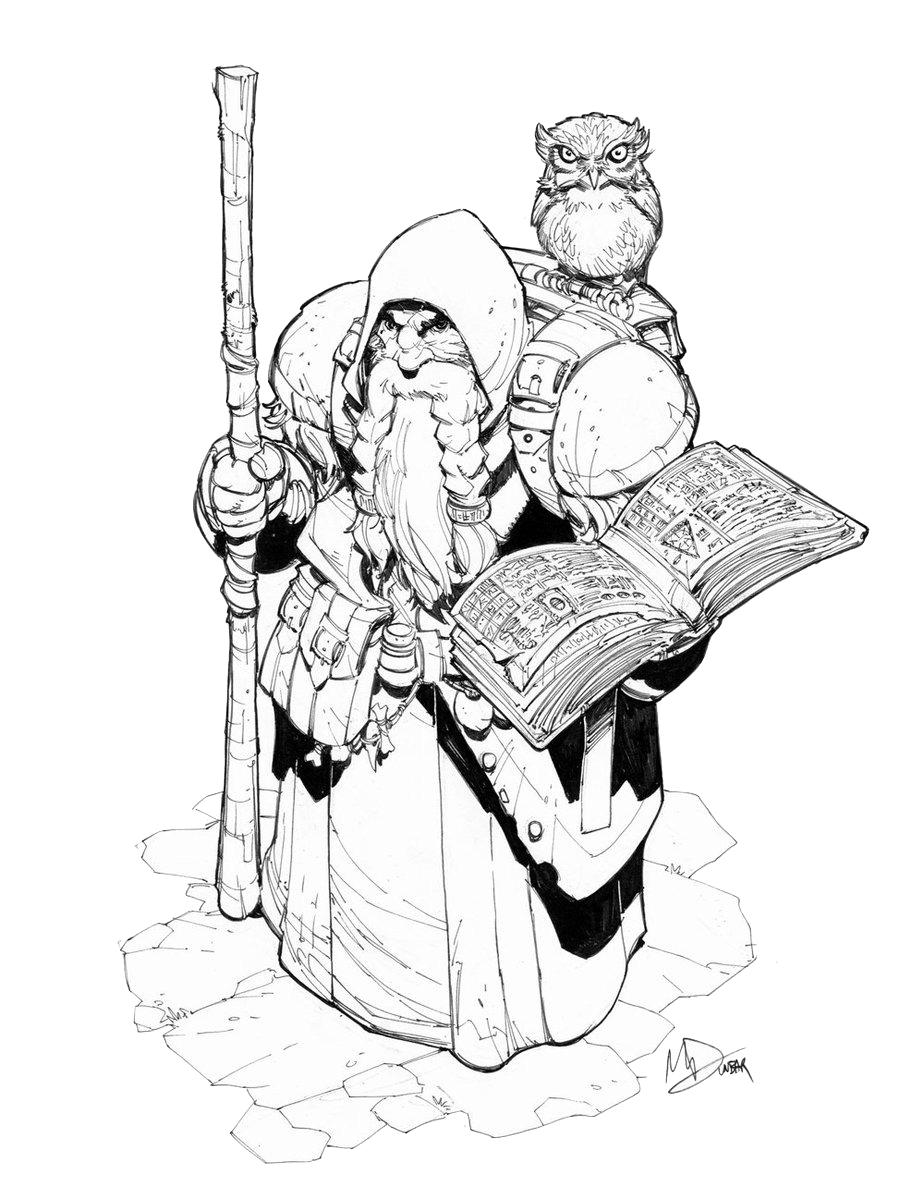
\includegraphics[width=\textwidth]{img/wizard-2.png}
{\scriptsize Art by Max Dunbar}
\end{Figure}
    
\end{multicols*}

    